\iffalse
\begin{SCfigure}
\begin{minipage}{0.65\textwidth}
\setlength{\unitlength}{0.65\textwidth}
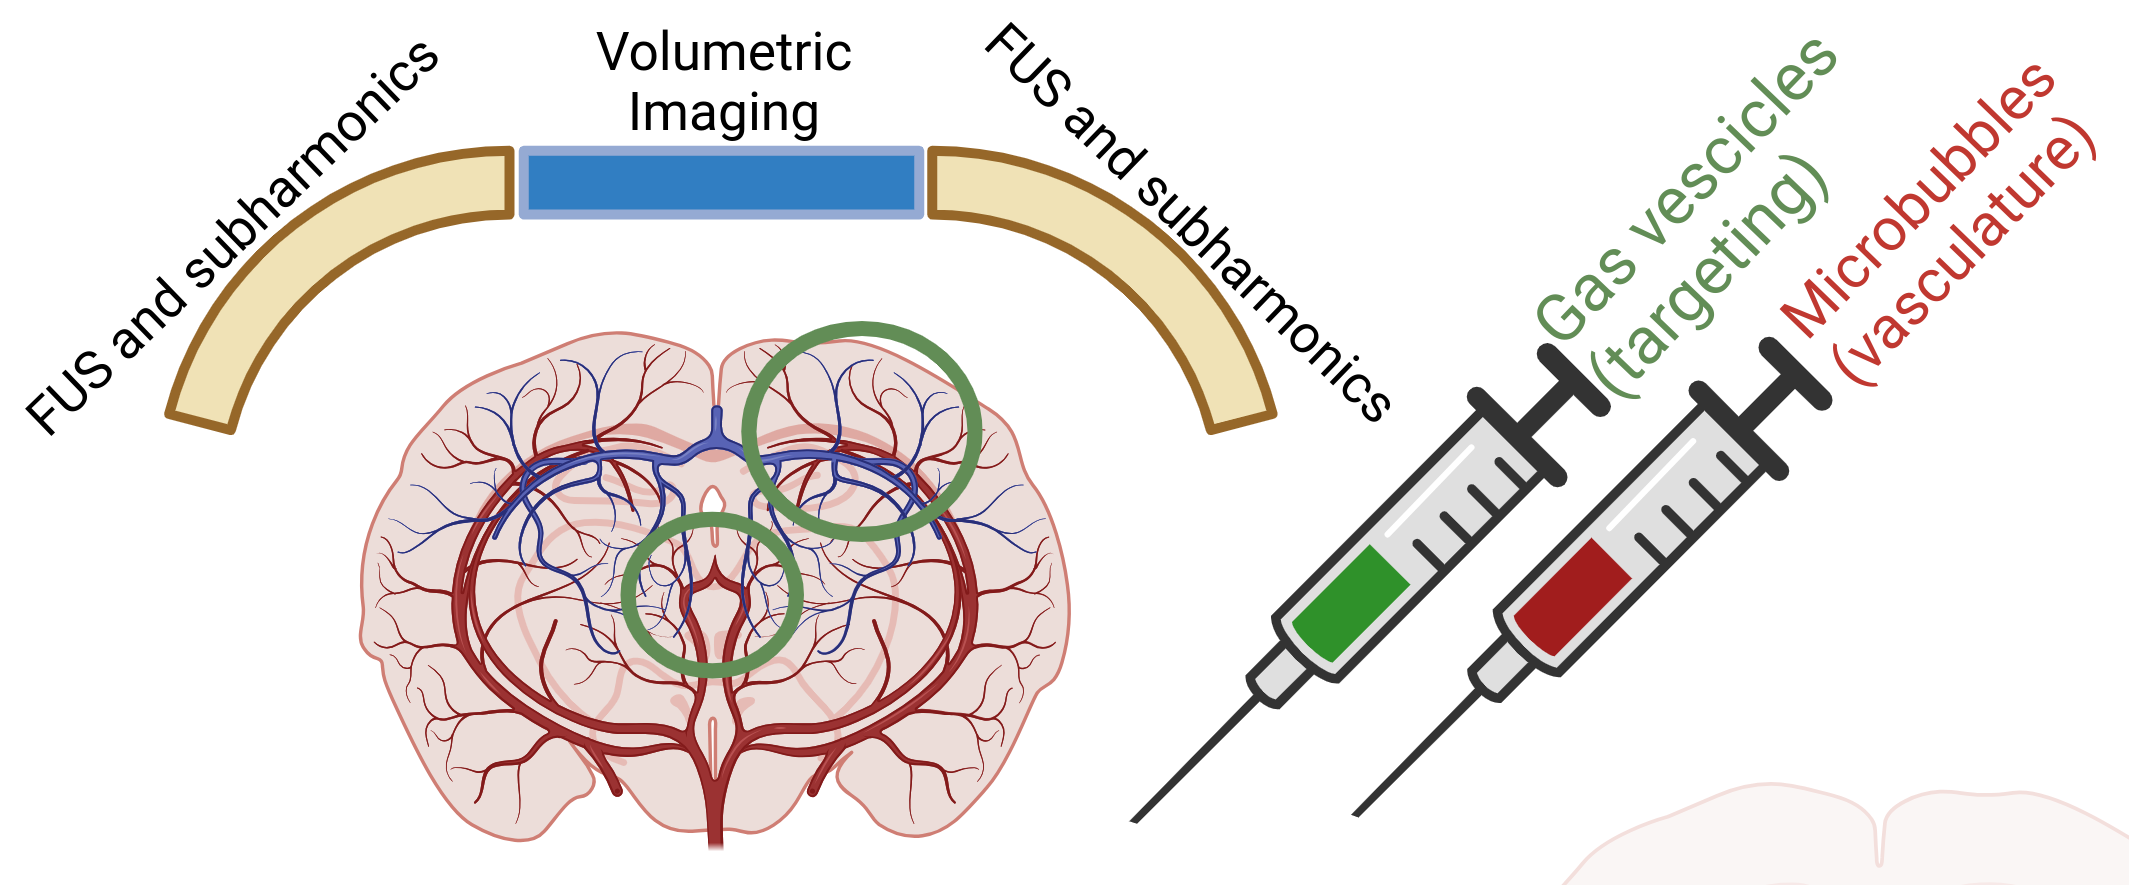
\includegraphics[width=\textwidth]{figures/approach_schematic.png}
\vspace{-10mm}
\end{minipage}
\caption{\textbf{Summary of image-guided surgical approach approach.} High frame-rate volumetric ultrasound is developed to image the whole-brain neurovasculature and targeted  response to injury using a single neuroimaging tool. (A) High frame-rate volumetric bmUS of first 500 ms image local VSSRA biomechanics  (B). From -10 min to 0 min (pre-injury baseline) and from 500 ms to 240 minutes post-injury the brain is monitored continuously with fUS sequences that image neurovascular response (D) and neurofunctional connectivity response (C). \vspace{-5mm}}
\label{fig:approach_summary}
\end{SCfigure}

\fi
Our approach focuses on developing and demonstrating the proposed technology for non-invasive ultra-high precision ultrasound imaging and targeted sonothrombolysis in the brain. Non-invasive volumetric whole-brain super-resolution ultrasound imaging with freely circulating microbubble contrast agents will characterize the neurovasculature with up to $10 \mu$m spatial resolution, enabling detection and localization of vascular occlusion and quantification of hemodynamic changes associated with stroke. Transcranial ultrasound arrays that deliver therapeutic sonothrombolytic pulses as well as low-frequency super-harmonic imaging transmits will be designed with custom transcranial wave propagation tools. Once fabricated we will implement imaging sequences that work in conjunction with existing matrix imaging arrays for non-invasive volumetric super-harmonic super-resolution ultrasound imaging. The combined imaging and therapy approach will be developed and validated first in rodent stroke models. Translation to human-scale acoustics will be achieved through extensive transcranial human phantom experiments and calibrated digital acoustic human models, reducing the need for large animal studies. Unpublished preliminary results establish feasibility in four key areas: non-invasive volumetric super-resolution microvascular imaging and quantification, transcranial imaging through thick skulls approximating human thickness, transcranial human imaging, and stroke detection in a rodent model.

\subsubsection{Unpublished preliminary results showing non-invasive whole-brain volumetric super-resolution for microvascular imaging and quantification: \label{sec:superres_microvascular}} Building on our recent work demonstrating that non-invasive fully volumetric ultrasonic imaging can assess microvascular changes during the longitudinal evolution of neurological disease in mice (Fig.~\ref{fig:gbm})~\cite{mccall2023longitudinal}, we show here that 1) individual vessels are identifiable non-invasively and transcranially, including critical vessels in healthy tissue, 2) their microvascular velocity and flow characteristics are quantifiable (Fig.~\ref{fig:gbm_quantification}), and 3) longitudinal changes in vascular morphology can be tracked. For example, analysis of microvascular hemodynamics shows that identifiable vessels have an average diameter of 77~$\mu$m and velocity of 30~mm/s in week 1, with measurable changes in diameter (101~$\mu$m), velocity (29~mm/s), and flow by week 2. This quantitative microvascular characterization---vessel identification, diameter, velocity, and flow---is directly applicable to detecting vascular occlusion, mapping the ischemic penumbra, and monitoring reperfusion during sonothrombolysis.

\subsubsection{Unpublished preliminary results: transcranial volumetric imaging with a unique human-scale sparse array.\label{sec:sparse_gv}} A custom 1024-channel 1.5~MHz ultra-wide (65~mm) sparse volumetric imaging array designed for human transcranial volumetric imaging was used to image contrast agents under a human skull (Fig.~\ref{fig:sparse_gv}). Focused amplitude modulation sequences achieve high contrast with respect to a tissue-mimicking background gel
\begin{wrapfigure}{l}{0.4\textwidth}
\vspace{5mm}
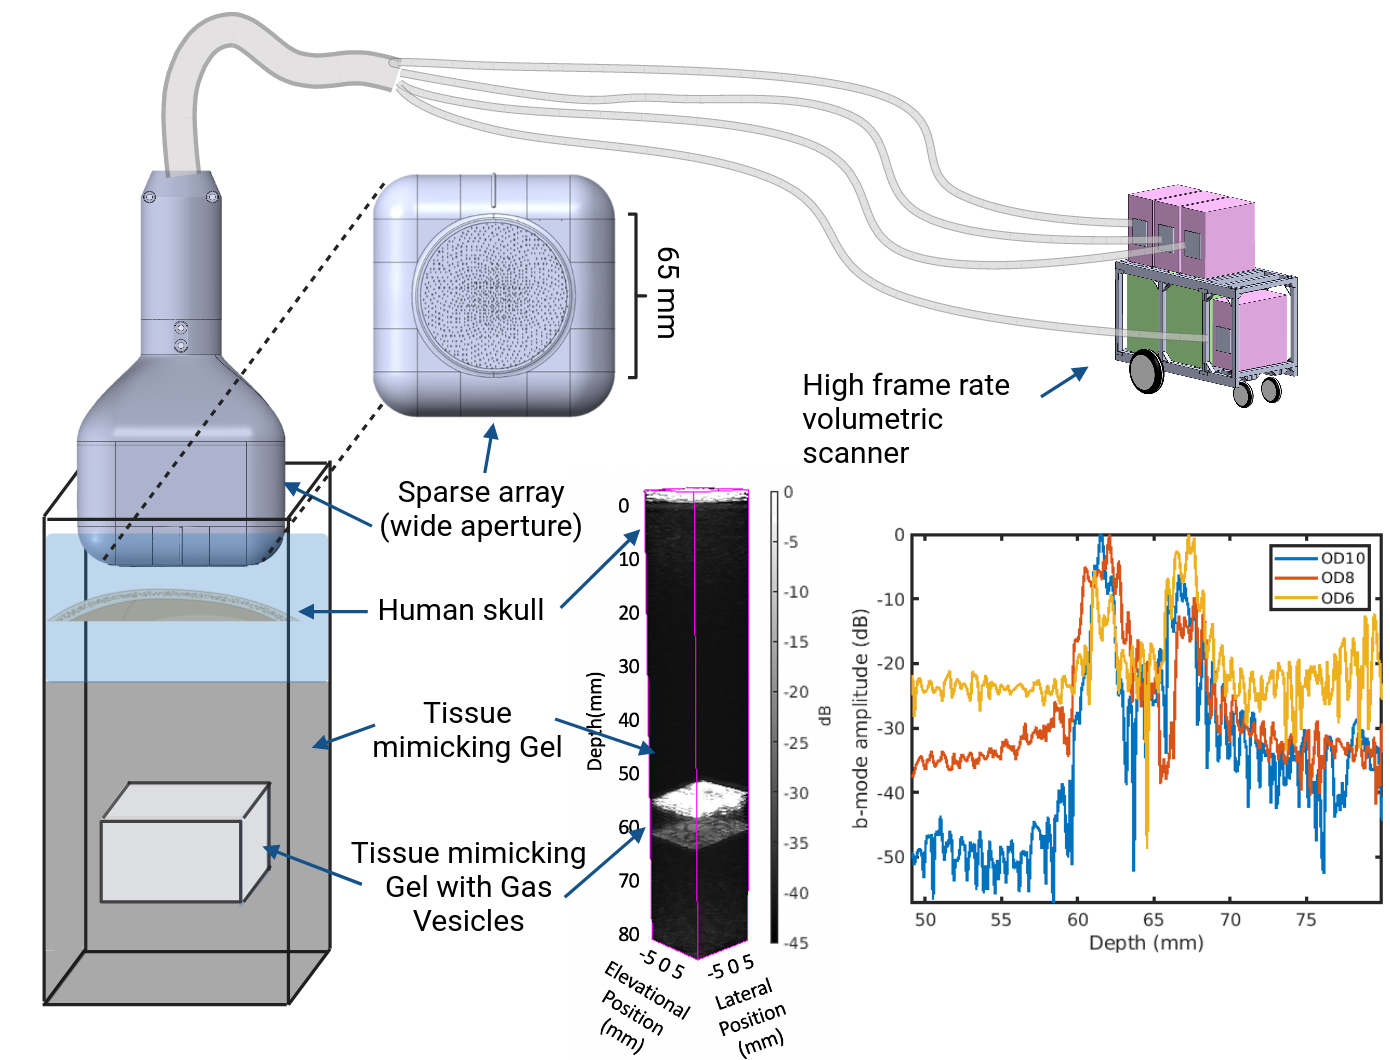
\includegraphics[width=0.4\textwidth]{figures/GV_sparse_array_schematic_v4.png}
\caption{\label{fig:sparse_gv} \textbf{Transcranial human-scale imaging.} A custom sparse 1.5~MHz imaging array with an ultra-wide 65~mm aperture designed for human transcranial volumetric imaging is used to image contrast agents under a human skull. Custom focused amplitude modulation sequences achieve high contrast with respect to a tissue-mimicking background gel (20~dB contrast at low concentrations).}
\vspace{-0cm}
\end{wrapfigure}

(20~dB contrast at low concentrations, and 40--50~dB at higher concentrations). To acquire these images, contrast agents were embedded in gelatin and placed at 65~mm below the transducer, with a piece of human temporal bone placed in between the transducer and gelatin. Focused imaging was used to create a 1.2~cm $\times$ 1.2~cm grid of 400 focal points at two different focal depths, performed at two consecutive pressures for amplitude modulation. This unique transducer achieves an aperture that is far larger than conventional matrix probes using a density-tapered spiral design sparse arrangement to significantly decrease grating lobes. The large aperture enables acquisition over a large field of view with a significant depth of more than 100~mm. Because of the large surface area, this probe can capture over 3 coherence lengths in each dimension and is therefore more effective when considering and correcting for aberrating environments, which is optimal for human transcranial imaging~\cite{mccall2023development}.

\subsubsection{Unpublished preliminary results: transcranial super-resolution imaging through thick skulls.}
The skull thickness of large dog breeds~\cite{o2017investigation} is similar to human thickness~\cite{o2017investigation,de2016human,lynnerup2005thickness}, making them an appropriate acoustic phantom for evaluating human translational feasibility. Preliminary results in a large-breed canine skull with a 380~$\mu$m cellulose microtube inserted in the skull cavity demonstrate the feasibility of super-resolution imaging transcranially through human-thickness bone (Fig.~\ref{fig:K9Skull}). We compared a custom fully-focused (FF) transmit super-resolution approach to conventional plane-wave compounding (PWC), both implemented on a Philips P4-1 transducer. The FF approach generated better contrast, enabling better penetration and localization counts. The microtube diameter estimates are $640~\mu$m for PWC and $420~\mu$m for FF, the latter corresponding closely to the known microtube size. These results establish feasibility of transcranial super-resolution at human-relevant skull thicknesses and depths.

\subsubsection{Unpublished preliminary results: transcranial human imaging.}
\hlc[myyellow]{PLACEHOLDER: Describe preliminary transcranial human imaging results here. Include figure reference, imaging parameters, and key metrics (resolution, contrast, depth).} These imaging techniques, combined with the human-scale sparse array described above~\cite{mccall2023development}, are poised for translation to \textit{in vivo} applications. \hlc[myyellow]{This unique transducer achieves an aperture that is far larger than conventional matrix probes using a density-tapered spiral design sparse arrangement to significantly decrease grating lobes compared to a dense matrix array probe. The large aperture of this probe also enables acquisition over a large field of view with a significant depth of more than 100~mm. Because of the large surface area of this probe, it can capture over 3 coherence lengths in each dimension and is, therefore, more effective when considering and correcting for aberrating environments which is optimal for human transcranial imaging.}

\subsubsection{Unpublished preliminary results: stroke detection in a rodent thromboembolic model.}
\hlc[myyellow]{PLACEHOLDER: Describe preliminary results from the in situ thrombin injection stroke model (thrombin injected into MCA via micropipette through craniotomy). Include imaging results showing detection of occlusion and/or perfusion changes, and relevant figure reference.} Building on our recent work demonstrating that non-invasive fully volumetric ultrasonic imaging can assess microvascular changes longitudinally (Fig.~\ref{fig:gbm})~\cite{mccall2023longitudinal}, we show here that \hlc[myyellow]{1) the thromboembolic occlusion significantly modifies the vascular morphology in the MCA territory, 2) occluded and partially occluded vessels are identifiable, as are critical vessels in healthy tissue and in the contralateral hemisphere, 3) their microvascular velocity and flow characteristics are quantifiable before and after occlusion.} \hlc[myyellow]{For example, analysis of the microvascular hemodynamics shows that PLACEHOLDER: insert quantitative metrics---vessel diameter, velocity, flow changes pre- vs post-occlusion, comparison of affected vs contralateral hemisphere, penumbral perfusion reduction.} This quantification enables detection and localization of the thrombus as well as characterization of the penumbral region, which is essential for guiding targeted sonothrombolysis while sparing vessels in healthy tissue.

\begin{wrapfigure}{r}{1.0\textwidth}
\vspace{-5mm}
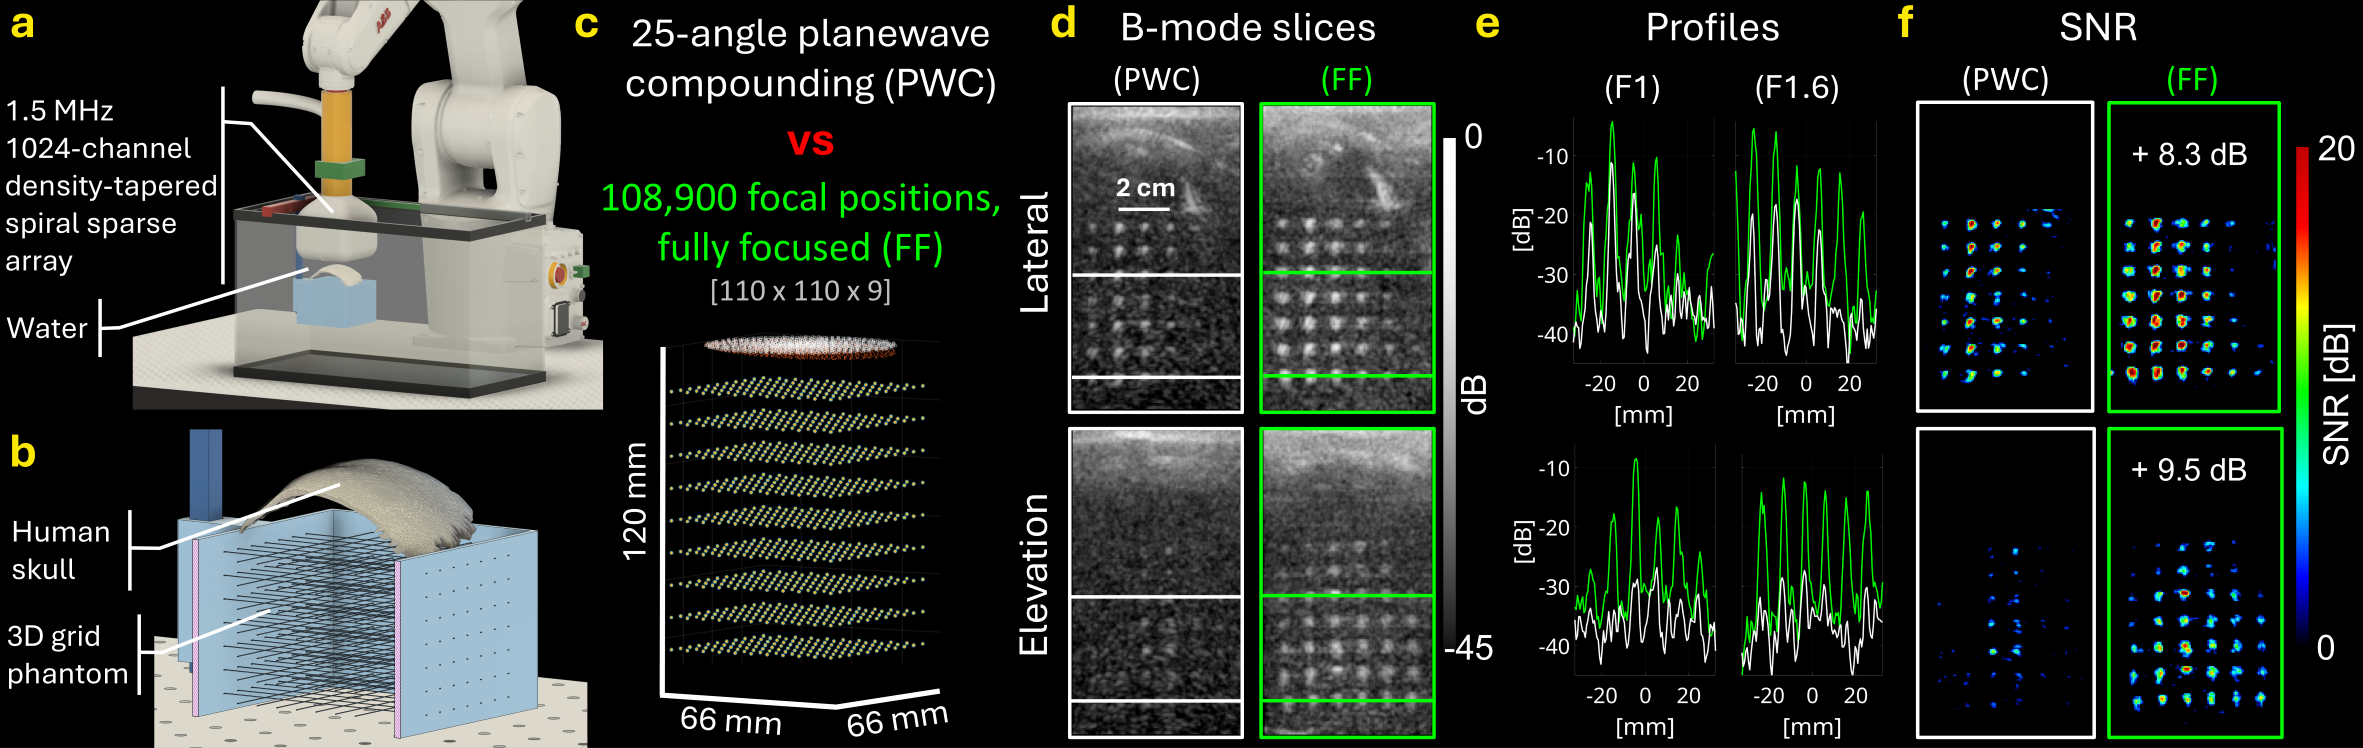
\includegraphics[width=1.0\textwidth]{figures/IUS_2025_ABSTRACT_Hatim3_V3_25percent.png}
\caption{Human transcranial imaging.}
\vspace{-3mm}
\end{wrapfigure}

\begin{wrapfigure}{hr}{0.5\textwidth}
\vspace{0mm}
    \centering
    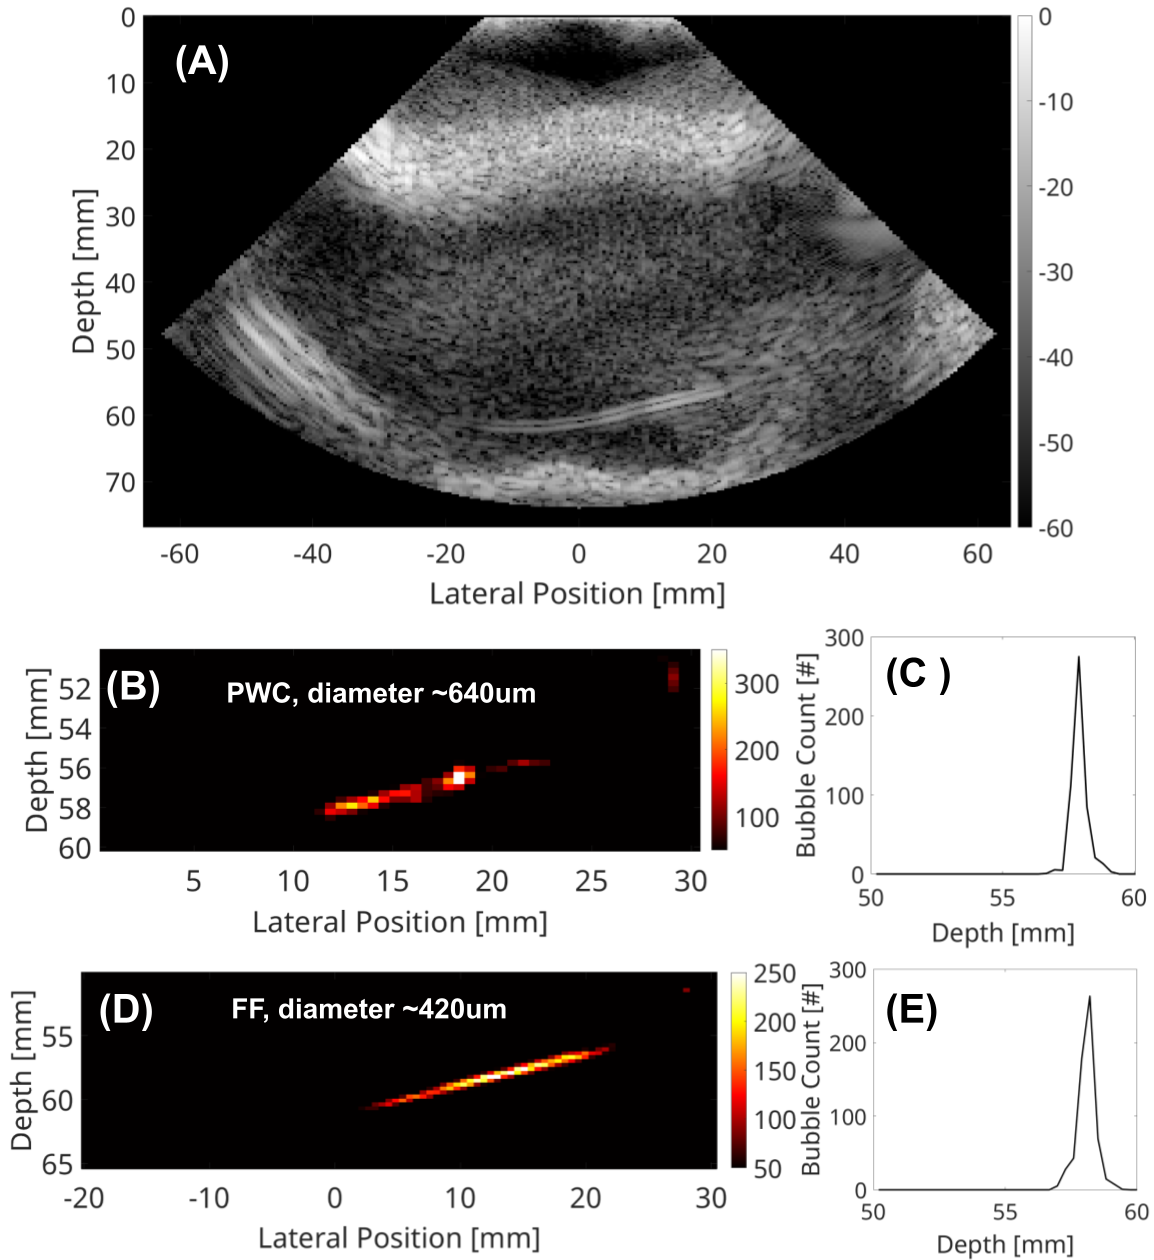
\includegraphics[width=0.5\textwidth]{figures/K9Skull_Combined.png}
    \vspace{0mm}\caption{\label{fig:K9Skull} Preliminary results demonstrating feasibility of focused transcranial super-resolution through a thick skull with human-like thickness. (A) Transcranial B-mode image of a $380~\mu$m tube. (B) Super-resolution imaging using PWC. (C) Measured vessel diameter is $640~\mu$m. (D) Super-resolution imaging using FF. (E) Measured vessel diameter is $420~\mu$m, in close agreement with real size.}
    \vspace{0mm}
\end{wrapfigure}
\begin{wrapfigure}{hr}{0.5\textwidth}
\vspace{-5mm}
    \centering
    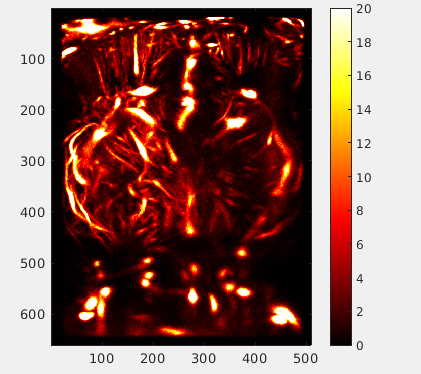
\includegraphics[width=0.5\textwidth]{figures/Stroke.png}
    \vspace{-8mm}\caption{placeholder until better images finish processing (pre/post, velocity, etc.)}
    \vspace{-5mm}
\end{wrapfigure}

\subsubsection{Animal models for stroke.}
\textbf{Justification:} The thromboembolic stroke model produces a fibrin-rich thrombus that occludes the middle cerebral artery territory, closely mimicking the pathophysiology of human ischemic stroke~\cite{orset2007mouse,niessen2003thromboembolic,carmichael2005rodent}. Unlike the intraluminal filament model, which produces mechanical occlusion without a clot, the thromboembolic model generates a real thrombus that can be dissolved by thrombolytic agents and sonothrombolysis, making it the most appropriate model for evaluating therapeutic recanalization~\cite{andjus2024preclinical}. Key features include: reproducible infarcts in the MCA territory when optimized, clinically relevant clot composition (fibrin and platelets), compatibility with rt-PA thrombolysis and sonothrombolysis protocols, and the ability to monitor recanalization and reperfusion with imaging. The model also produces an ischemic penumbra with salvageable tissue surrounding the infarct core, enabling evaluation of the therapeutic time window. We will use the \textit{in situ} thrombin injection model~\cite{orset2007mouse}, in which $\alpha$-thrombin is injected directly into the MCA lumen via a micropipette to form a clot \textit{in situ}. A micropipette is prepared using a moving-coil microelectrode puller and loaded with human $\alpha$-thrombin (4~UI/$\mu$L). The rat is placed in a stereotactic frame and a vertical incision is made between the eye and ear. The temporal muscle is retracted, the skull is thinned, and a craniectomy is performed to expose the MCA bifurcation. A laser Doppler probe is placed over the MCA territory for continuous cerebral blood flow (CBF) monitoring. The micropipette is inserted into the MCA lumen through the bifurcation and $\alpha$-thrombin is slowly injected to induce clot formation. The pipette is left in place for a minimum of 20 minutes to allow clot stabilization, then withdrawn. Successful occlusion is confirmed by a stable CBF drop of $\geq$65\% for 1 hour. This model produces highly reproducible and localized occlusions with low mortality ($\sim$2\%) and is compatible with rt-PA thrombolysis, making it ideal for controlled evaluation of sonothrombolytic efficacy. The craniotomy will be performed with care to preserve bone fragments for acoustic replacement or a thin cranial window approach to maintain an acoustic pathway for transcranial imaging and therapy. As an alternative, the embolic clot injection model~\cite{niessen2003thromboembolic}---in which a pre-formed autologous blood clot is delivered intravascularly via the external carotid artery through the internal carotid artery to the MCA origin---leaves the skull fully intact, preserving the acoustic environment for transcranial ultrasound. However, this model has higher mortality ($\sim$16\%) and greater variability in infarct size. If the thrombin injection model proves incompatible with transcranial imaging due to the craniotomy, the embolic clot injection model will be adopted.
The collaborative development of volumetric super-resolution imaging and targeted sonothrombolysis \textbf{(SA1)} and characterization of \textit{in vivo} stroke detection and therapeutic efficacy will be validated in this animal model \textbf{(SA2)}.
\textbf{Number of small animals to be used:} We estimate 98 rats will be required for statistical significance in the imaging and therapy tasks (\ref{sec:imaging_optimization1}, \ref{sec:thermal_validation}, \ref{sec:agent_optimization}): 20 for \textit{in vivo} super-harmonic imaging optimization with microbubbles, 20 for stroke detection and microvascular characterization with the thromboembolic model, 10 for \textit{in vivo} contrast agent formulation validation (\ref{sec:agent_optimization}), and 48 for sonothrombolysis efficacy evaluation across six groups ($n=8$ per group: image-guided sonothrombolysis with combined microbubble/nanodroplet formulation, image-guided sonothrombolysis with microbubbles only, ultrasound-only, agents-only, IV tPA positive control, and untreated stroke). This model will establish the relationship between a) super-resolution detection of vascular occlusion and perfusion changes, b) targeting accuracy of focused sonothrombolysis, c) degree of recanalization and reperfusion achieved, and d) validation with histology (TTC staining for infarct volume, H\&E for hemorrhage) and conventional imaging.
\textbf{Translation to human-scale acoustics:} Rather than relying on large animal models, we will validate the translational feasibility of transcranial imaging and therapy through extensive human skull phantom experiments and calibrated digital acoustic human models. Fullwave 2 simulations~\cite{pinton2009heterogeneous,pinton2021fullwave} driven by CT-derived skull maps will model transcranial propagation, aberration, and therapeutic focusing in anatomically realistic human head models. These digital acoustic humans, calibrated by our small animal \textit{in vivo} results and human phantom measurements, will predict imaging and therapeutic performance at human scale while substantially reducing the need for large animal experimentation.
\textbf{Sex and age as a biological variable:} Animals of both sexes will be used in equal numbers. All statistical analyses will be conducted both in the population aggregate and with sex stratification, to explore any potential modification by sex as a biological variable.


\subsection{Specific Aim 1: Develop and implement volumetric non-invasive transcranial contrast-enhanced super-resolution dual-frequency imaging methods that detect stroke and quantitatively characterize the microvascular environment.}


\begin{wrapfigure}{hr}{0.5\textwidth}
\vspace{-5mm}
    \centering
    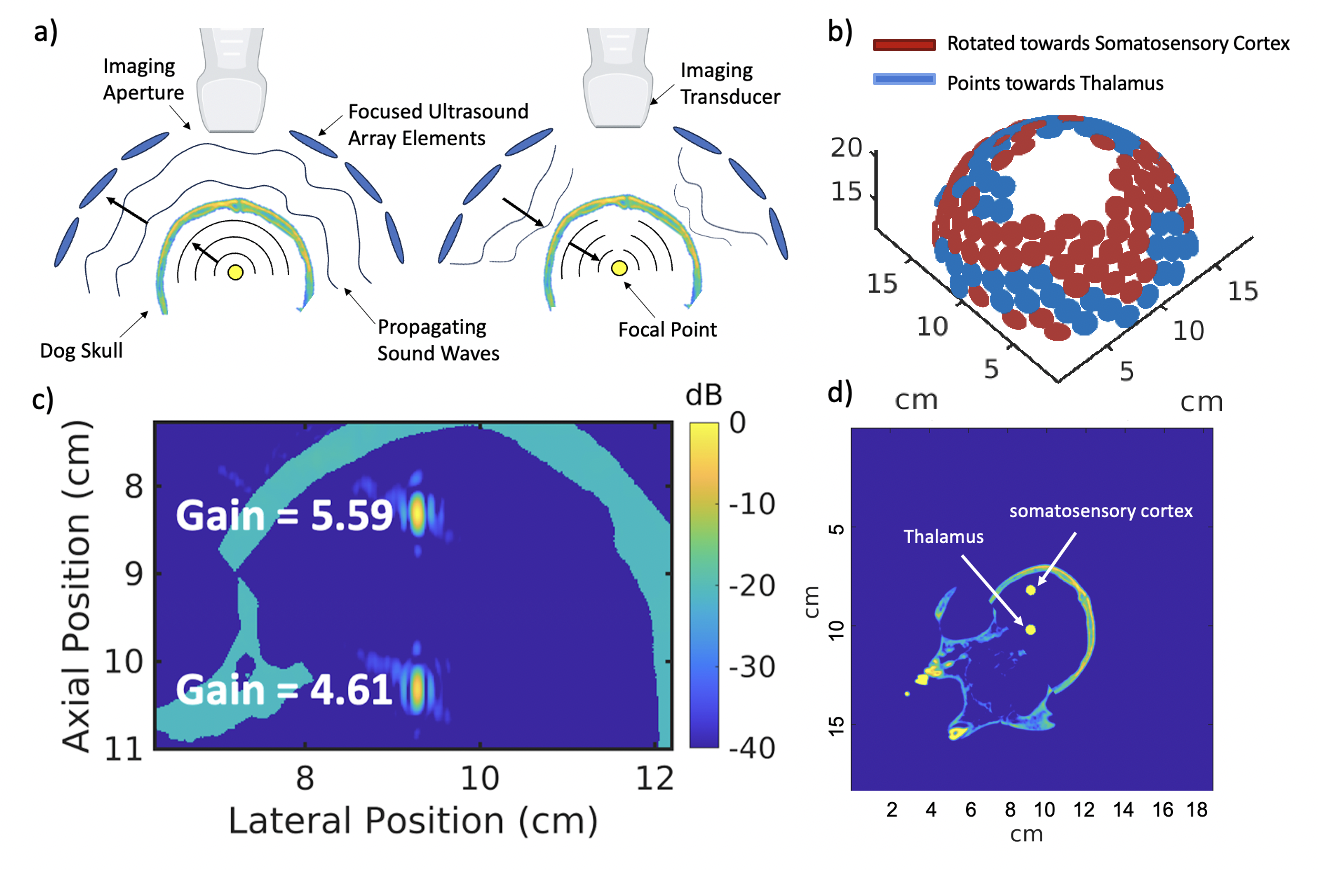
\includegraphics[width=0.5\textwidth]{figures/SR_fUS_array.png}
    \vspace{-8mm}\caption{\label{fig:NeuromodArray}\textbf{Dual-frequency array designs for combined transcranial imaging and therapy} (A) Fullwave 2 time reversal simulations are used to correct phase aberration and determine optimal transducer placement. (B) Optimized geometry for multifocal transmit from an array with an imaging void. (C-D) Focal gains for simultaneous neuromodulation of somatosensory and thalamic targets~\cite{jones2021transcranial}}
    \vspace{-5mm}
\end{wrapfigure}
\subsubsection{Develop outrigger array that acts both as a super-harmonic source and as a therapeutic source. \label{sec:xducer_design}}
\textbf{Rationale:} Our previous implementations of super-harmonic imaging have been in 2D. Advances in the dual-frequency transducer technology and optimization of the system parameters are critical for acquiring 3D transcranial super-harmonic images. Further optimization is required to satisfy constraints for therapeutic transmits which will be delivered by the same outrigger array. \textbf{Methods:} Two outrigger arrays, for small and large animals, will be designed using the similar tools and principles we have used previously in ultrasound neuromodulation arrays for nonhuman primates and human transcranial imaging arrays~\cite{jones2021transcranial,mccall2023development}.
\textbf{Small animal array system:} will consist of an existing Vermon 8 MHz 1024-channel matrix array which will act as the receive beamforming aperture. It is paired with a new custom 128-channel tapered spiral directional hemispherical array with a 2 MHz center frequency, 30\% bandwidth, 20 mm imaging hole, and 100 mm total width (quote from Imasonic included). 
\textbf{Human transcranial array system:} will consist of an existing 1.5 MHz custom 1024-channel, 65 mm aperture sparse array that we have designed and built in collaboration with Daxsonics for transcranial imaging in humans (Fig.~\ref{fig:sparse_gv})~\cite{mccall2023development}. It is paired with a new custom 128-channel tapered spiral directional hemispherical array with a .65 MHz center frequency, 30\% bandwidth, 65 mm imaging hole, and 150 mm total width (quote from Imasonic included).
Five Verasonics systems will be used simultaneously to drive an array pair. Four systems comprising 1024 channels will drive the matrix imaging probes, and an extended power supply 256 channel system will drive the outrigger arrays.\textbf{ \textit{In silico} design and optimization:} will be performed with 3-D Fullwave 2 simulations~\cite{pinton2009heterogeneous,pinton2021fullwave} that will optimize the outrigger element position, size, and frequency so that the arrays can: 1)  steer and focus to targets within the brain volume 2) can attain sufficient focal gains for effective sonothrombolytic delivery at the target and 3) include an imaging aperture for super-resolution imaging. Optimization will be performed  separately for murine and human skulls. These simulations include the effects of the skull based on acoustical maps derived from  CTs and $\mu$CTs~\cite{Aubry2003,aubry2010high,pinton2009phase}. They are used to calculate the acoustical path through species (rats) or patient-specific (human) skulls by exploiting the time-reversal invariance of the wave propagation~\cite{fink1992time,pinton2009phase}. A result of this time-reversal process includes the correction of aberration induced by the skull~\cite{tanter1998focusing,pinton2009nonlinear_a}.  The element orientation is not to a single focal spot, rather the design integrates multiple orientations of elements so that subgroups focus to different locations. This overcomes directional constraints of large elements. The design shown in Fig.~\ref{fig:NeuromodArray} is based on a spherical array, with 128 15-mm elements distributed in a spherical helix pattern.  Spherical arrays have good focusing capabilities through the skull at the center of the array, but focusing on off-center locations is more challenging due to the natural geometric configuration and the angle of incidence with the skull. To mitigate this, the elements closest to the aperture were rotated toward and focusing on shallow targets, and the 64 elements farthest from the aperture were rotated toward and focusing on deeper targets. This optimization resulted in an array design that can focus on the somatosensory cortex with a gain of 5.19 and the thalamus with a gain of 4.4.  This array and beam design processes will be adapted for small animals ($\sim$2 MHz) and humans ($\sim$ 650 kHz) with additional considerations of focal spot size, reverberation, standing wave effects, and array size. \textbf{Characterization:} will be performed \textit{in silico} then experimentally  in a water tank  when the arrays are delivered using standard acoustical characterization techniques, including 3D beam mapping, mechanical index, thermal index, peak pressure, side-lobe height, voltage/pressure sensitivity, and angular sensitivity measurements. These measurements will also enable calibrated acoustical dose estimates in subsequent treatment planning (\ref{sec:thermal_validation}). \textbf{Outcome:} Optimized low frequency outrigger arrays with an imaging hole that can deliver both super-harmonic transmits and therapeutic transmits within the brain volume of small animals and human-scale phantoms. Quotes for these two arrays are provided by Imasonic, a world-leader in custom array fabrication. 




\begin{wrapfigure}{hr}{0.45\textwidth}
\vspace{0mm}
    \centering
    %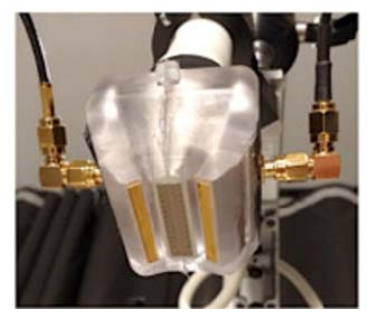
\includegraphics[width=0.15\textwidth]{figures/Screenshot from 2023-10-14 09-54-47.png}
    %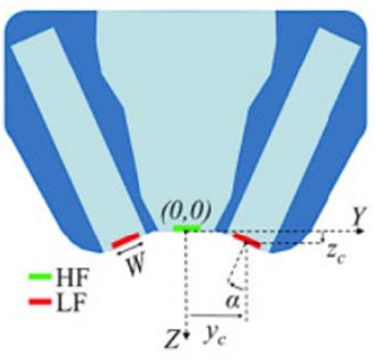
\includegraphics[width=0.15\textwidth]{figures/Screenshot from 2023-10-14 09-54-57.png}
     %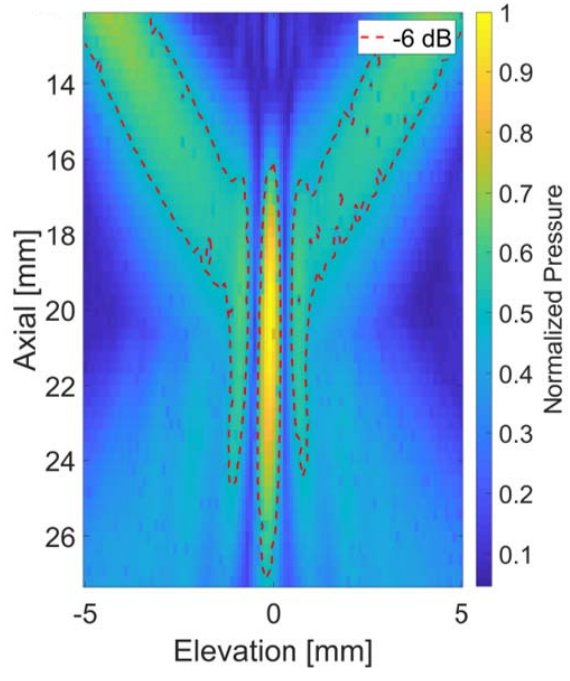
\includegraphics[width=0.15\textwidth]{figures/Screenshot from 2023-10-14 09-55-04.png}

    \rotatebox[origin=c]{90}{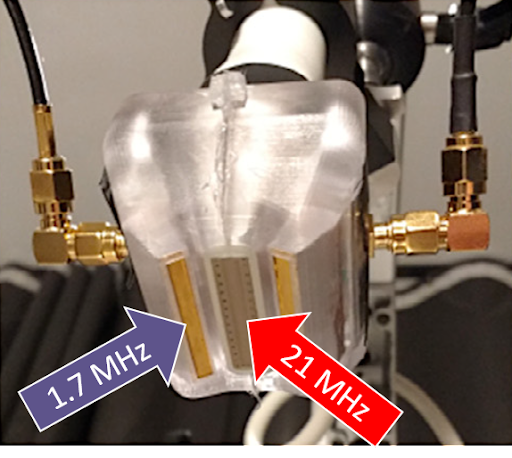
\includegraphics[width=0.22\textwidth]{figures/df_xducer.png}}
  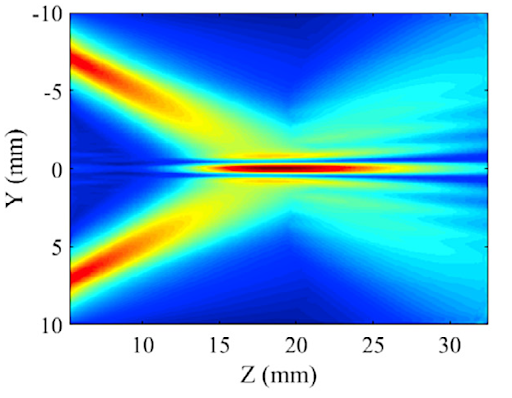
\includegraphics[width=0.22\textwidth]{figures/df_field.png}
  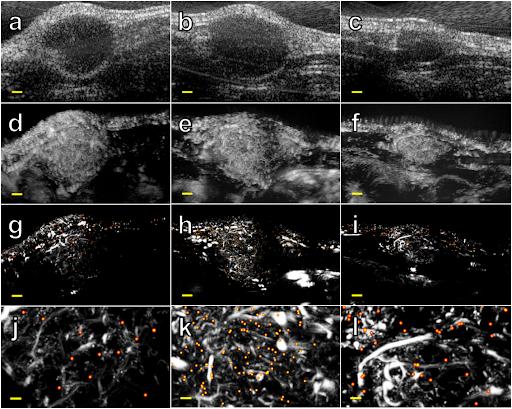
\includegraphics[width=0.44\textwidth]{figures/df_targeting.png}
  \begin{picture}(0,0)(240,-10)
    % left-column
    \put(2,140){\tiny{\textcolor{yellow}{1 mm}}}
    \put(2,93){\tiny{\textcolor{yellow}{1 mm}}}
    \put(2,45){\tiny{\textcolor{yellow}{1 mm}}}
    \put(2,-2){\tiny{\textcolor{yellow}{250 $\mu$m}}}
    % central-column
    %\put(83,140){\tiny{\textcolor{yellow}{$250\mu m$}}}
    %\put(83,93){\tiny{\textcolor{yellow}{$250\mu m$}}}
    %\put(83,45){\tiny{\textcolor{yellow}{$250\mu m$}}}
    %\put(83,-2){\tiny{\textcolor{yellow}{$250\mu m$}}}
    % right-column
    %\put(162,140){\tiny{\textcolor{yellow}{$250\mu m$}}}
    %\put(162,93){\tiny{\textcolor{yellow}{$250\mu m$}}}
    %\put(162,45){\tiny{\textcolor{yellow}{$250\mu m$}}}
    %\put(162,-2){\tiny{\textcolor{yellow}{$250\mu m$}}}
    \end{picture}
    \vspace{-0mm}\caption{\label{fig:df} \textbf{Imaging of stationary and free-flowing contrast agents with super-harmonic ultrasound} (Top row) An outrigger dual frequency linear probe with 1.7 MHz transmit and 20 MHz receive capabilities. The acoustical field generated by low frequency transmits. Super-resolution ultrasound molecular imaging in three rodent fibrosarcomas. (a-c) B-mode images from the center of each tumor captured with the high-frequency elements of the dual-frequency array (dynamic
range = 40 dB). (d-f)  Super-harmonic B-modes images acquired across
the tumor volumes (dynamic range = 30 dB). (g-i) Super-harmonic super-resolution ultrasound
localization microscopy of free-flowing microbubbles (gray colormap) with super-resolved signaling of targeted microbubbles overlaid (warm colormap, localizations are
blurred to improve visibility, true size is smaller). Scale bars are 1 mm. (j-l) 2 mm x 3.5 mm selections from each super-resolved image
showing microvascular and biomarker detail. Scale bars are 250 µm. 
(Adapted from ~\cite{kierski2020superharmonic,kierski2022acoustic}) } %***annotate scale bars in image*** done!
     \vspace{-5mm}
\end{wrapfigure}
\subsubsection{Develop super-resolution super-harmonic transcranial imaging methods \textit{in silico}.\label{sec:imaging}} Imaging design and optimization will occur in three phases, \textit{in silico}, \textit{in vitro} and \textit{in vivo} (\ref{sec:imaging_optimization1}).
\textbf{Rationale:}  Microbubble response is highly nonlinear as a function of pressure amplitude. High contrast imaging depends on  sequences that exploit this nonlinearity. In preliminary studies, we have combined super-harmonic super-resolution imaging with targeted microbubble contrast agents to  obtain super-resolved 3D maps of blood vessels and locations of molecular activity in a rat fibrosarcoma model (Fig.~\ref{fig:df})\cite{kierski2020super,kierski2022acoustic}. We seek to advance this work to detect both free-flowing and stationary microbubbles near a vascular occlusion, enabling quantitative characterization of the microvascular environment in stroke.
 \textbf{Methods:} \textit{In silico} superharmonic imaging performance will be carried out by simulating excitation of microbubbles via the Marmottant model~\cite{marmottant2005model} across a range of acoustic pressures and frequencies and calculating the scattered acoustic content from these microbubbles. Imaging performance will be estimated by calculating the contrast-to-tissue ratio (CTR) of the microbubble signal from higher order harmonic content, which can be captured within the transducer bandwidth. This contrast signal will be compared to the anticipated nonlinear tissue content from the excitation pulse, as calculated using 3D angular spectrum code combined with a Rusanov method (ASR) that we designed for accurate nonlinear wave evolution~\cite{luo2020rapid}. Scattered acoustic responses will be simulated for transmit frequencies in the range of 0.5 – 3 MHz, for bubbles with radii similar to Definity~\cite{goertz2007attenuation}. Transmit waveforms with variable frequency and pressure will be generated as an input to the ASR simulations. Fullwave 2 simulations will be used to model the effects of heterogeneous propagation in the skull and brain~\cite{pinton2009heterogeneous,pinton2021fullwave}. This multi-scale multi-physics approach allows us to combine the nonlinear attenuating wave propagation physics from the nonlinear contrast agent response. CTR will then be optimized within the receive bandwidth of each dual frequency transducer pair. Preliminary results demonstrate that the Marmottant and ASR models can be used in combination to create an \textit{in silico} metric of CTR. Simulation results for a 1.5 $\mu$m bubble, excited with a 4 MHz transmit at 2 cm depth and received at 25 – 30 MHz, are shown in Fig.~\ref{fig:df_sims}. These preliminary data agree with our previous experimental studies~\cite{newsome2020visualization,newsome2021implementation} which have measured CTR between 15 – 30 dB with DF wobbler probes.
\textbf{Outcome:} Optimized transmit amplitude and acoustical parameters for dual-frequency imaging through murine and human skulls.


\subsubsection{Imaging optimization. \label{sec:imaging_optimization1}} \textbf{\textit{In vitro:}} optimization will be performed for freely flowing microbubbles.  DF contrast imaging experiments with microbubbles will be performed in a skull phantom with and tissue mimicking gel containing 100 $mu$m diameter microtubes ~\cite{espindola2018adaptive,soulioti2019super}. In-house microbubbles will be infused using a syringe pump at a given set of low frequency drive parameters (transmit pulse shapes, mechanical index,
\begin{wrapfigure}{l}{0.25\textwidth}
\vspace{0mm}
    \centering
    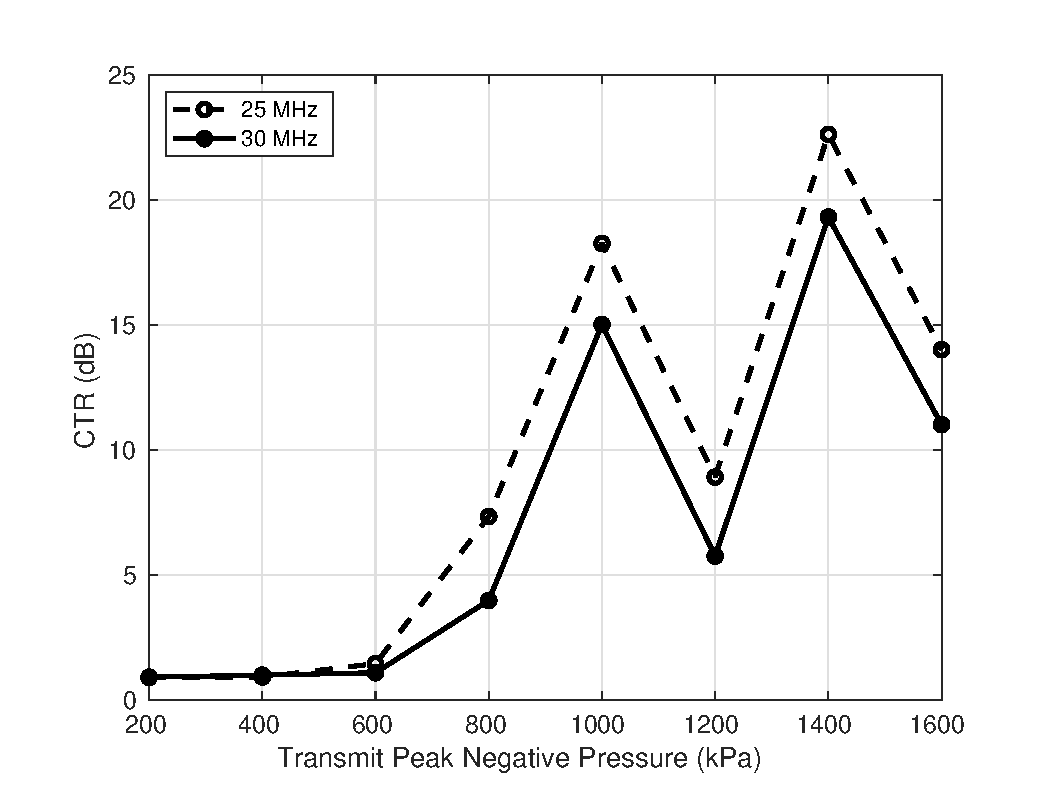
\includegraphics[width=0.25\textwidth]{figures/sims_fig_1600.eps}
    \vspace{-5mm}\caption{\label{fig:df_sims} \textbf{Theoretical predictions of CTR for design and optimization.} Simulation results for a 1.5 $\mu$m bubble, excited with a 4 MHz transmit at 2 cm depth and received at 25 – 30 MHz.}
    \vspace{-5mm}
\end{wrapfigure}
etc) as previously described~\cite{lindsey2014acoustic}. Driving criteria optimized by previous tasks \textit{in silico} (\ref{sec:imaging}) will be validated here.
 \textbf{\textit{In vivo:}} optimization will be performed in 20 rats for microbubble imaging optimization. An iterative simulation (\ref{sec:imaging}) validation approach will be used. Unlike conventional super-resolution sequences, super-harmonic super-resolution sequences do not rely on SVD-based spatial temporal sequences~\cite{christensen2020super} and  may benefit from different compounding since the frame-rate requirements are less stringent. Thus transmit-receive and beamforming optimization performed using:  Hadamard encoding to improve the SNR in plane-wave compounding~\cite{tiran2015multiplane,rabut20194d}, reconstruction of synthetic aperture transmits which combines the advantages of focusing and compounding~\cite{bottenus2018refocus}, parallel receive beamforming with fully focused or  partially focused beams to reduce skull reverberation and off-axis clutter~\cite{shattuck1984explososcan,chandrasekaran2022situ}, and nonlinear harmonic and pulse inversion imaging, driven by the low frequency transducer,  which may further suppresses tissue signal and enhance contrast agent signal~
\cite{simpson1999pulse,Tranquart1999,pinton2009heterogeneous,brown2019investigation}. \textbf{Success metrics:} The detected super-harmonic content, contrast-to-tissue ratio (CTR), signal-to-noise ratio (SNR), and resolution will be evaluated as a function of driving variables, as per prior work~\cite{gessner2010high,mccall2021characterization}. Focused imaging sequences will be evaluated for human skull phantoms (Fig.~\ref{fig:K9Skull}). A subset of experiments will be performed where human skull segments are placed in front of transducer to introduce degradation while imaging the rat brain with the human-scale transducer pair.
 \textbf{Outcome:} We will identify the optimal transmit-receive imaging sequences and acoustical parameters for transcranial super-harmonic imaging in rats and human skull phantoms.
%***Include amplitude modulation where outrigger is used simultaneously to imaging pulse (essentially the 2 MHz does the amplitude modulation, while the 8 MHz does the imaging).
 
\subsubsection{\textit{In silico} and \textit{in vitro} characterization of sonothrombolysis and validation of sonothrombolytic treatment planning: \label{sec:thermal_validation}} Murine and human head phantoms will characterize the pressure fields inside the brain and the performance of the outrigger transducers operating in therapeutic mode. \textit{In silico}, the same CT and $\mu$CT from \ref{sec:xducer_design} that were converted into maps of the acoustical properties will be used to model ultrasound propagation using Fullwave 2, including pressure field characterization, mechanical index mapping, and cavitation threshold modeling as we have performed previously~\cite{zhao2005two,pinton2011attenuation,pinton2011cavitation,pinton2009phase}. Our group has developed specialized transducer designs for sonothrombolysis, including forward-viewing intravascular transducers~\cite{kim2017intravascular,goel2021safety} and multi-pillar piezoelectric stack transducers~\cite{kim2021multi}, providing extensive experience in transducer-clot interaction characterization. Experimental characterization will be performed with skull phantoms consisting of murine or human skulls containing clot-mimicking phantoms (blood clot in microtube inside skull phantom) embedded in tissue mimicking gel. Cellulose (SigmaAldrich) is added as a scattering and attenuating agent in concentrations that vary around 1\% depending on the desired attenuation properties.
Microbubbles will be infused at their expected \textit{in vivo} concentrations. Post sonothrombolytic treatment, clot dissolution rate and residual clot mass will be measured to characterize the therapeutic efficacy and to validate the simulation tools. Passive cavitation detection will be used to monitor cavitation activity during treatment.
\textbf{Success metrics:} Transmit properties, including the pulse length, duration, number of focal zones, and location will be characterized in terms of peak negative pressure, mechanical index, and cavitation dose at the target location in the brain and at the skull surface both \textit{in silico} and \textit{in vitro}. Infrared cameras and thermocouples will monitor the skull surface to ensure thermal safety as we have done previously~\cite{pinton2011attenuation}. Adjustments to material properties in simulations, such as skull absorption or effective tissue absorption, will be performed to match experimental measurements and aid in subsequent calibrated sonothrombolytic treatment planning. \textbf{Outcome:} Characterization of pressure fields and cavitation activity as a function of acoustical parameters and validation of simulation tools for sonothrombolytic treatment planning.

\subsubsection{Robotic compounding to remove shadowing, improve image quality, and determine targeting window.\label{sec:robotic_compounding}} 
\textbf{Rationale:} Skull structures such as sutures and crests as well as variations in the thickness create shadow regions that reduce image quality and penetration of therapeutic pulses. \textbf{Methods:} We have developed a robotic compounding approach to place the transducer on different parts of the skull surface to obtain volumetric images of the same volume but from different points of view (Fig.~\ref{fig:robot}). In these non-invasive transcranial volumetric super-resolution images, shadowing is apparent in different regions of the brain. These different volumes are then averaged together using standard 3D non-rigid image registration techniques (MATLAB, imregdeform). Preliminary results illustrate the technique using a high precision (10 $\mu$m positional accuracy) ABB IRB 120 industrial robot which we have programmed to position a Vermon 8 MHz matrix array to five registered locations on the surface of an \textit{in vivo} rat head. Non-invasive transcranial volumetric super-resolution imaging sequences~\cite{mccall2023non} were used to acquire data (Fig.~\ref{fig:robot}). Each angle takes 2.5 minutes to acquire. Each individual volume has different regions of shadowing, but the registered averaged volume shows how vessels re-populate with   robotic compounding. 
\begin{wrapfigure}{r}{0.55\textwidth}
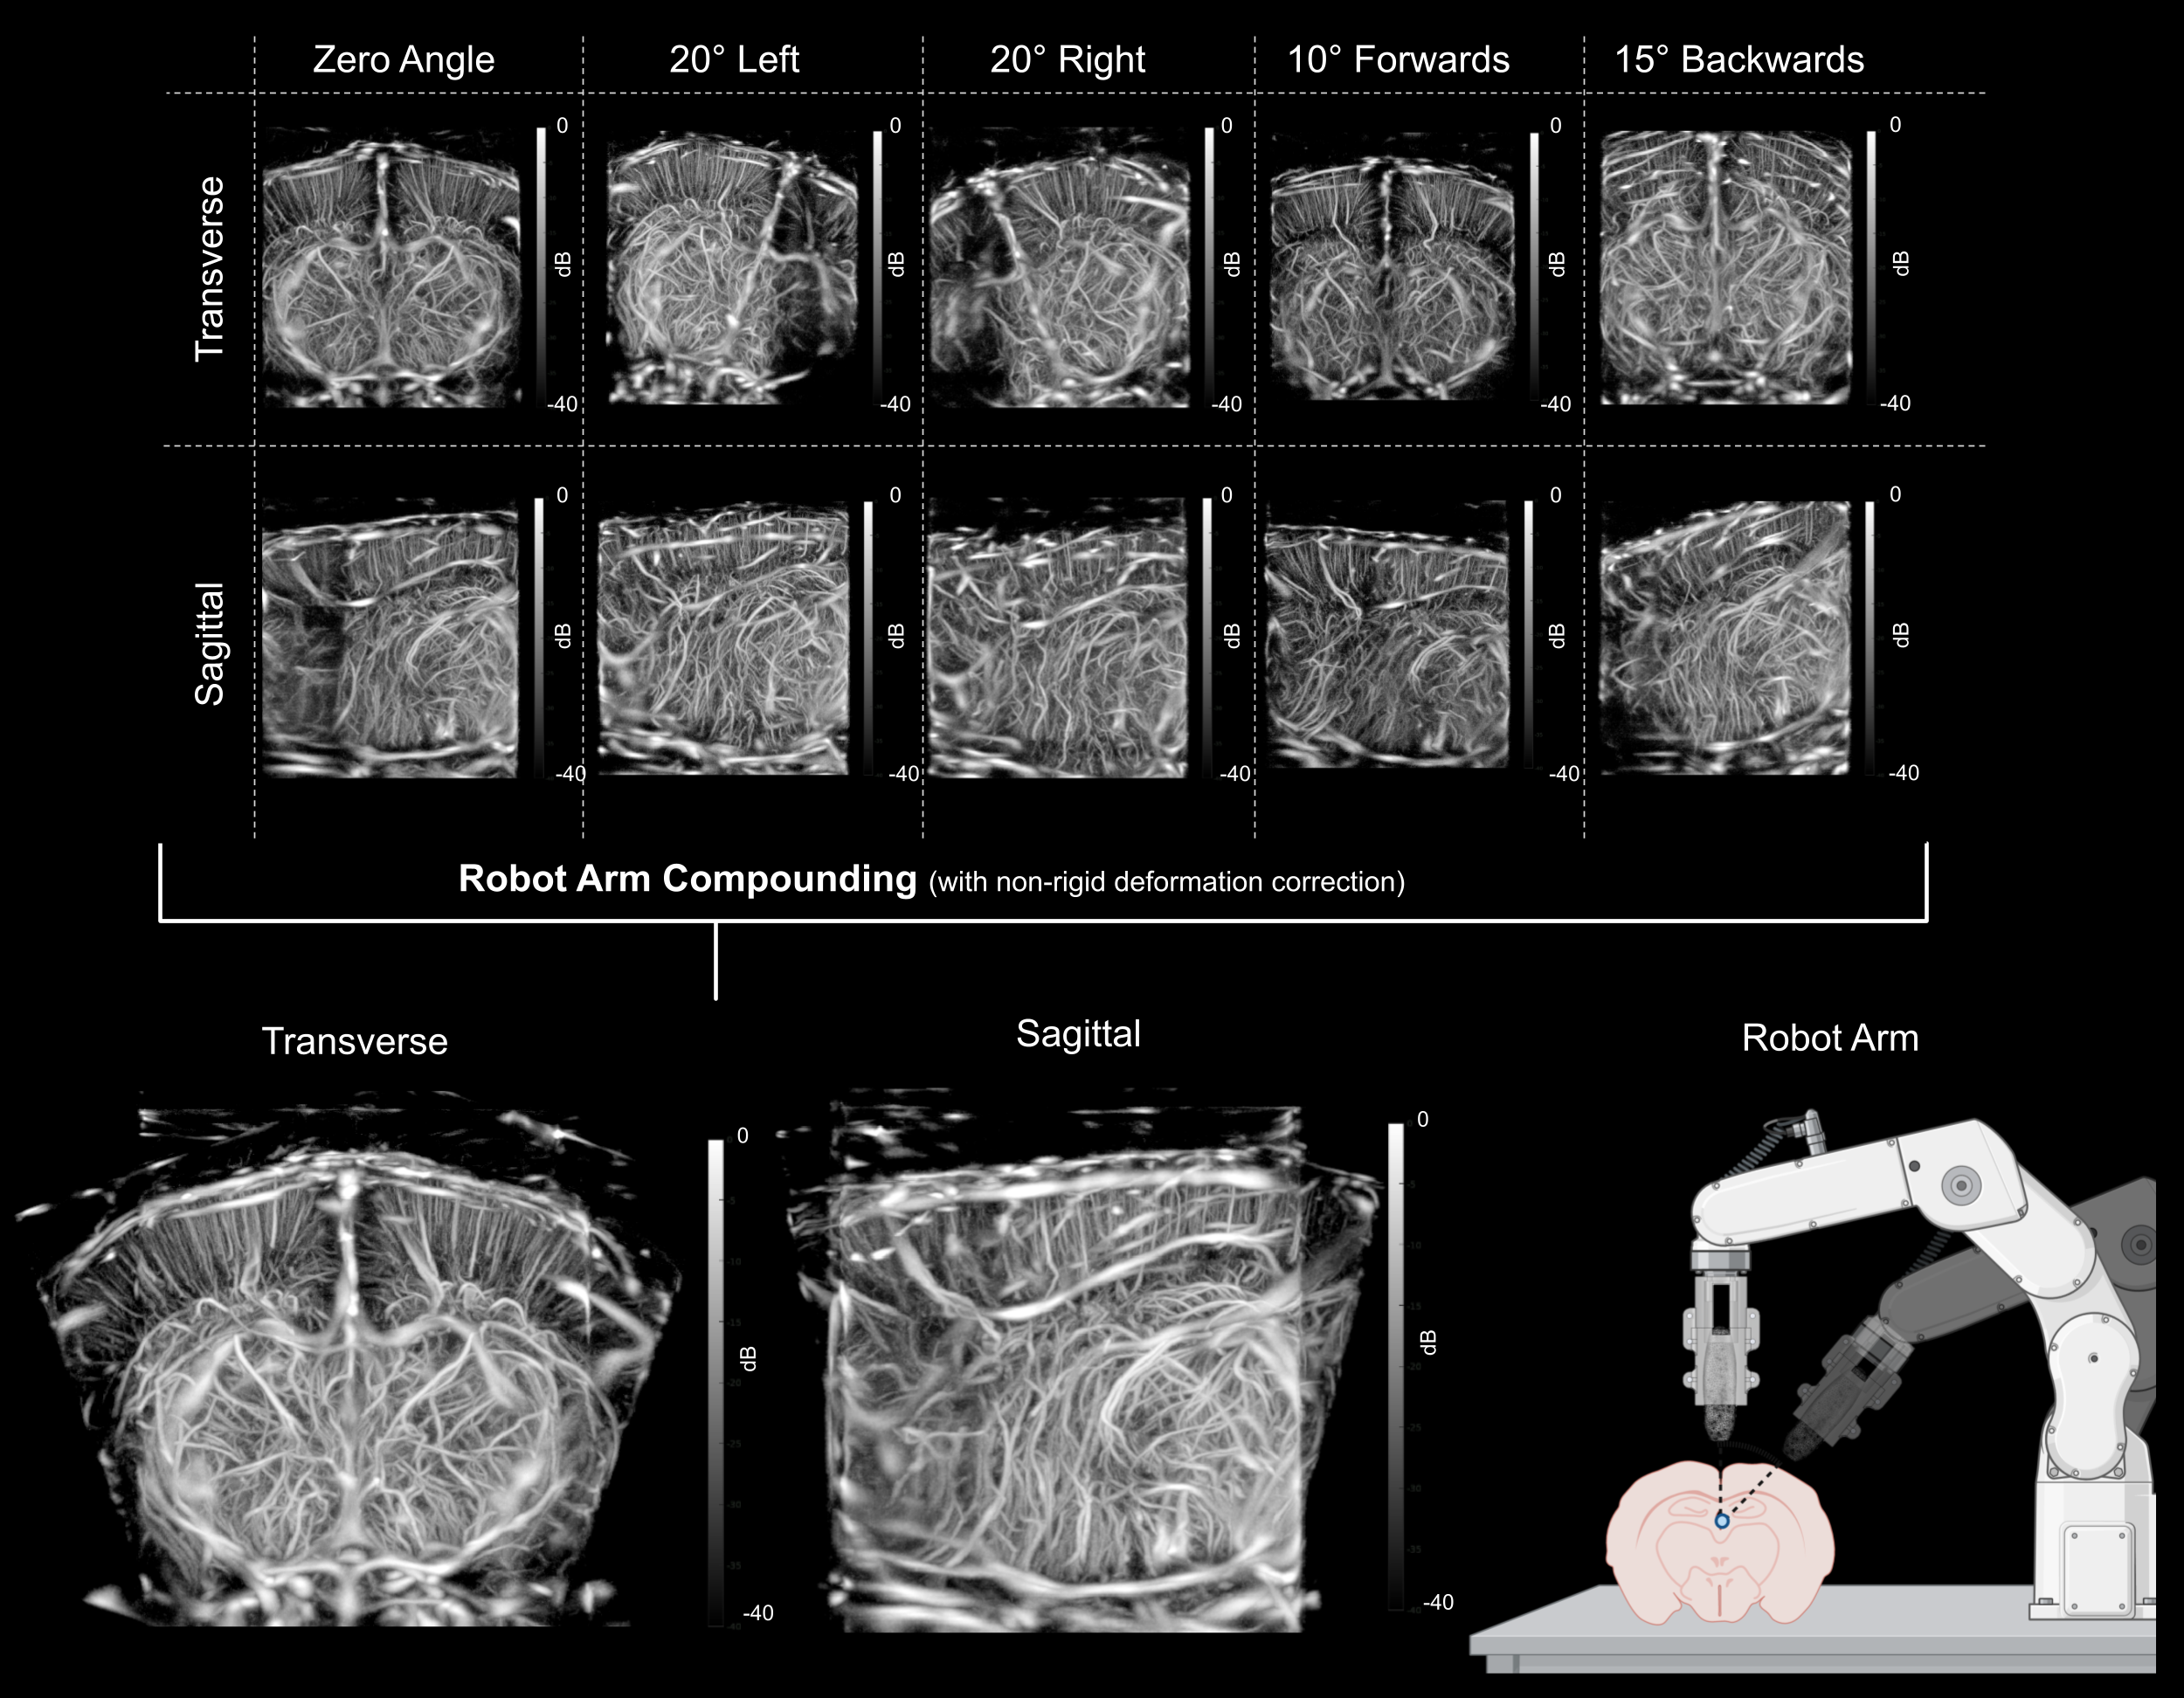
\includegraphics[width=0.55\textwidth]{figures/RobotArmCompounding_Fig3.png}
\caption{\label{fig:robot} \textbf{Robotic compounding in non-invasive transcranial volumetric super-resolution imaging in the rat brain.} Shadowing is apparent in individual angles (top row). Compounding using non-rigid registration approaches removes shadowing and improves image quality (bottom).}
\vspace{-0cm}
\end{wrapfigure}
This approach also allows us to determine acoustical windows that are optimal for therapy by ensuring that the stroke/occlusion region is not shadowed. \textbf{Success metrics:} Improved image quality measured by vessel SNR and resolution \textit{ex vivo} and \textit{in vivo}. Improved therapeutic targeting measured by pressure delivery and therapeutic focal volume with skull phantoms. Both murine and human-scale transducers will be tested. \textbf{Outcome:} robotic compounding approaches improve image quality and determine optimal cranial window for imaging/FUS.

\subsubsection{Rapid acquisition and processing.\label{sec:rapid}} \textbf{Rationale:} volumetric super-resolution generates massive amounts of data, on the order of 24 Gb/s, resulting in tens of terabytes over a typical 2-hour imaging session. Rapid turnaround is required for targeting \textit{in vivo} within the anesthesia window. \textbf{Methods:} We have over 6 years of experience using the 1024-channel Verasonics system and have built highly efficient data management and processing tools resulting in the fastest published acquisition times of any group~\cite{mccall2023non}. For a high-quality super-resolved 100,0000 volume the data acquisition and transfer time is currently 2.5 minutes and our processing time is 30 minutes on 4 $\times$ Nvidia GTX 3090 using our custom beamformers and processing code.  \textbf{Outcome:} Continued innovation on fast GPU beamforming, high-speed data management, and high-quality imaging to rapidly generate volumetric super-resolution images for targeting. 

\subsubsection{Validate super-resolution imaging in thromboembolic rat stroke model.} The thromboembolic rat stroke model will be used to validate super-resolution imaging for stroke detection and microvascular characterization. \textbf{Methods:} Non-invasive super-harmonic super-resolution sequences will acquire images of vascular morphology before and after stroke induction. Imaging will demonstrate detection of the vascular occlusion, microvascular characterization of the ischemic penumbra, and quantification of flow changes associated with stroke. Quantitative microvascular analysis (\ref{sec:superres_microvascular}) will be used to characterize changes in vessel density, tortuosity, and flow velocity in the penumbral region. Serial imaging will track the evolution of the ischemic territory over time. After the procedure the brain will be fixed and validated with subsequent histology including TTC staining for infarct delineation and H\&E for tissue characterization~\cite{hurt2023genomically,bar2021acoustically}. \textbf{Success metrics:} Success will be measured by detection sensitivity for vascular occlusion, correlation of super-resolution imaging with histological infarct boundaries, and quantification of penumbral perfusion changes. Successful detection of occlusion in $>$80\% of stroked rats, and significant correlation between SR-derived microvascular metrics and histologically confirmed infarct volume.
\subsubsection{Pitfalls and alternative strategies} 
Coded excitation optimized based on nonlinear microbubble signature may be implemented to increase contrast. A smaller number of volumes may be acquired to more rapidly generate super-resolved images and targeting. Large microbubbles (2-4$\mu$m) may be fabricated in-house via filtration to augment contrast. If the thromboembolic stroke model proves too variable, alternative models such as photothrombotic or endothelin-1 injection models will be used. If super-harmonic CTR is insufficient through the skull, alternative imaging sequences such as amplitude modulation or contrast pulse sequences will be investigated.

\subsection{Specific Aim 2: To develop therapeutic sonothrombolysis for image-guided treatment of stroke.}
We will develop a combined ultrasound system that delivers both imaging and therapeutic beams through the intact skull. The dual-frequency outrigger arrays developed in SA1 (\ref{sec:xducer_design}) will operate in interleaved imaging and therapy modes: super-harmonic imaging transmits will acquire volumetric super-resolution images to localize the thrombus and characterize the surrounding microvasculature, while therapeutic transmits will deliver focused sonothrombolytic pulses to the clot site. The \textit{in silico} and \textit{in vitro} sonothrombolytic characterization performed in SA1 (\ref{sec:thermal_validation}) establishes the acoustical parameters for safe and effective clot lysis. A central component of this aim is the optimization of ultrasound contrast agent formulations that serve the dual purpose of super-resolution imaging and sonothrombolysis. We will employ a class of agents that includes both conventional microbubbles and phase-change nanodroplets---sub-micron ($\sim$200~nm) liquid perfluorocarbon particles that upon acoustic activation convert to gas-filled microbubbles \textit{in situ}~\cite{bautista2023current}. While conventional microbubbles provide excellent imaging contrast and cavitation-mediated clot erosion at the thrombus surface, phase-change nanodroplets offer a complementary mechanism: their sub-micron size allows them to extravasate and penetrate into the fibrin matrix of the thrombus, where upon activation they generate microbubbles that cavitate from within the clot interior~\cite{kim2020comparison,goel2021nanodroplet}. Our prior work has demonstrated that the combination of conventional microbubbles and phase-change nanodroplets achieves optimal clot mass reduction that exceeds either agent alone~\cite{kim2022analysis}, motivating a systematic optimization of the agent formulation for the dual requirements of this theranostic platform. Here, we focus on the \textit{in vivo} therapeutic pipeline: contrast agent formulation optimization, real-time clot localization, image-guided delivery of sonothrombolysis, and evaluation of therapeutic efficacy in the thromboembolic rat stroke model.

\subsubsection{Optimization of dual-purpose contrast agent formulations for imaging and sonothrombolysis.\label{sec:agent_optimization}}
\textbf{Rationale:} The proposed theranostic platform requires contrast agents that simultaneously provide high-quality super-resolution imaging and potent sonothrombolytic enhancement. Conventional microbubbles (e.g., Definity, 1--3~$\mu$m diameter) are well-established for both super-resolution imaging and cavitation-enhanced thrombolysis, but their size restricts them to the vascular lumen where they erode the clot surface externally. Phase-change nanodroplets are a specialized formulation within the same perfluorocarbon contrast agent family: hundred-nanometer liquid droplets that convert to gas-filled microbubbles upon ultrasound activation at low acoustic energies~\cite{bautista2023current}. Their sub-micron size allows them to diffuse into the fibrin matrix of the thrombus, where ultrasound-triggered phase change generates microbubbles that cavitate internally, initiating clot breakup from within~\cite{kim2020comparison,goel2021nanodroplet}. This ``permeation and internal disruption'' mechanism produces clot dissolution in dense, retracted clots that is unachievable with conventional microbubbles or ultrasound alone~\cite{kim2022analysis}. Critically, our prior \textit{in vitro} studies demonstrate that the combination of conventional microbubbles and nanodroplets achieves optimal clot mass reduction that exceeds either agent alone~\cite{kim2022analysis}, as external cavitation from microbubbles and internal cavitation from activated nanodroplets act synergistically. \textbf{Methods:} We will systematically optimize the contrast agent formulation for the dual requirements of imaging and therapy. Low-boiling-point ($-2$\degree C) perfluorocarbon nanodroplets will be fabricated in-house using established protocols from the Dayton laboratory~\cite{kim2020comparison,bautista2023current}. The optimization will proceed in two stages:

\textit{Stage 1: In vitro formulation optimization.} Using the clot-in-tube phantom from \ref{sec:thermal_validation}, we will characterize: (a) the imaging performance (CTR, SNR, super-harmonic signal, localization count rate for super-resolution) and (b) the sonothrombolytic efficacy (percent clot mass reduction, cavitation dose) as a function of: microbubble concentration, nanodroplet concentration, and the microbubble-to-nanodroplet ratio. Imaging and therapy will use the dual-frequency array operating in interleaved mode with the optimized acoustic parameters from \ref{sec:thermal_validation}. The goal is to identify the agent formulation that maximizes both imaging quality and thrombolytic efficacy. We expect that a formulation enriched in microbubbles will favor imaging (higher nonlinear scattering) while a formulation enriched in nanodroplets will favor thrombolysis of retracted clots (greater internal penetration); the optimal dual-purpose formulation will balance these requirements.

\textit{Stage 2: In vivo formulation validation.} The top candidate formulations from Stage~1 will be validated \textit{in vivo} in the thromboembolic rat stroke model. Agents will be administered intravenously and the dual-frequency array will perform interleaved imaging and therapy. Super-resolution imaging quality will be assessed before and during therapy, while thrombolytic efficacy will be evaluated by imaging-based reperfusion metrics and post-mortem histological analysis. The \textit{in vivo} results will determine whether the agent concentrations and ratios that are optimal \textit{in vitro} translate to the \textit{in vivo} setting, where hemodynamic conditions, clot composition, and agent biodistribution introduce additional variables. These \textit{in vivo} agent characterization data will also inform the Fullwave~2 simulation models (SA3) by providing calibrated acoustic source terms for microbubble and nanodroplet populations under realistic conditions.

\textbf{Success metrics:} Identification of a dual-purpose agent formulation that achieves CTR within 80\% of the microbubble-only imaging benchmark while achieving $>$50\% clot mass reduction \textit{in vitro}. \textit{In vivo} validation demonstrating super-resolution imaging quality sufficient for clot localization concurrent with measurable thrombolytic effect. \textbf{Outcome:} An optimized, dual-purpose contrast agent formulation for integrated imaging and sonothrombolysis.

\subsubsection{Real-time clot localization and therapy guidance.\label{sec:clot_targeting}}
\textbf{Rationale:} Super-resolution imaging (SA1) can detect vascular occlusion and characterize the ischemic penumbra. For effective sonothrombolysis, the therapeutic focus must be accurately registered and guided to the clot location in real time. \textbf{Methods:} Because the imaging and therapeutic arrays share a common coordinate system through the dual-frequency array geometry, spatial registration between the imaging volume and the therapeutic focal zone is inherent. The imaging-to-therapy pipeline will operate as follows: 1) volumetric super-resolution imaging identifies the location of the occlusion based on the absence of microbubble flow and disrupted vascular morphology, 2) the therapeutic focal zone is electronically steered to the identified clot location using the time-reversal focusing approach from \ref{sec:xducer_design}, 3) sonothrombolytic pulses are delivered, and 4) follow-up imaging confirms clot disruption and monitors reperfusion. The robotic compounding system (\ref{sec:robotic_compounding}) will be used to position the array for optimal acoustical access to the occlusion site. Rapid acquisition and processing (\ref{sec:rapid}) will enable imaging feedback within the therapeutic time window. \textbf{Success metrics:} Targeting accuracy within 2~mm of clot center as validated by histological clot location, time to localization $<$~5~minutes from start of imaging. \textbf{Outcome:} A validated real-time clot localization and therapy guidance pipeline.

\subsubsection{Sonothrombolytic protocol optimization.\label{sec:sono_optimization}}
\textbf{Rationale:} Therapy parameters---mechanical index (MI), duty cycle, pulse repetition frequency (PRF), pulse duration, and treatment duration---critically affect thrombolysis efficacy and safety. Excessive acoustic pressure increases hemorrhage risk, while insufficient pressure fails to achieve recanalization. The optimized dual-purpose agent formulation from \ref{sec:agent_optimization}, combining conventional microbubbles with phase-change nanodroplets, provides two complementary cavitation mechanisms: microbubbles cavitate at the clot surface while activated nanodroplets cavitate within the clot interior~\cite{kim2022analysis,kim2020comparison}. This combined approach has been shown to achieve optimal clot mass reduction~\cite{kim2022analysis} and may enable effective thrombolysis at lower acoustic pressures than either agent alone, which is critical for transcranial applications where skull attenuation limits deliverable pressure. Additionally, dual-frequency ultrasound excitation has been demonstrated to produce significantly greater thrombolysis than single-frequency approaches at equivalent pressures~\cite{wu2021dual}, motivating the use of frequency mixing as a therapeutic strategy. \textbf{Methods:} Building on the \textit{in silico} and \textit{in vitro} characterization from \ref{sec:thermal_validation} and the optimized agent formulation from \ref{sec:agent_optimization}, we will optimize the sonothrombolytic protocol \textit{in vivo} in the thromboembolic rat stroke model. The dual-frequency array will deliver interleaved imaging and therapy sequences: low-frequency therapeutic pulses (0.5--2~MHz) at MI values ranging from 0.4 to 1.5 will be applied to the identified clot site, interleaved with super-harmonic imaging transmits to monitor clot status. The optimized microbubble/nanodroplet formulation will be administered intravenously. In addition to single-frequency insonation, dual-frequency mixing protocols---simultaneously transmitting at two frequencies through the outrigger array---will be evaluated, as our prior \textit{in vitro} results demonstrate that frequency mixing produces enhanced cavitation activity and superior clot lysis compared to single-frequency excitation~\cite{wu2021dual}. The interaction between acoustic parameters and agent formulation will be characterized: nanodroplet activation threshold, which depends on the perfluorocarbon boiling point and acoustic frequency, will be matched to the transcranial pressure levels achievable through the rat skull. Passive cavitation detection using the imaging array elements will monitor both stable and inertial cavitation activity during treatment, enabling discrimination between microbubble cavitation (predominantly at the clot surface) and nanodroplet-derived cavitation (within the clot matrix) based on their distinct spectral signatures~\cite{kim2022analysis,kim2020comparison}. Treatment duration will be varied from 5 to 30 minutes with periodic imaging to assess recanalization. \textbf{Success metrics:} Recanalization rate as a function of MI, treatment duration, and agent formulation; hemorrhage incidence (assessed by H\&E histology); and correlation between cavitation dose and therapeutic efficacy. Demonstration that the combined microbubble/nanodroplet formulation achieves superior recanalization compared to microbubbles alone at equivalent or lower acoustic pressures. \textbf{Outcome:} An optimized sonothrombolytic protocol---including acoustic parameters and agent formulation---that balances efficacy and safety for the thromboembolic rat model.

\subsubsection{\textit{In vivo} evaluation of image-guided sonothrombolysis.\label{sec:efficacy_study}}
\textbf{Rationale:} A controlled efficacy study is required to demonstrate that image-guided sonothrombolysis with the optimized dual-purpose agent formulation achieves superior outcomes compared to conventional approaches. \textbf{Methods:} Forty-eight rats with thromboembolic stroke will be randomized into six groups ($n=8$ per group): (1) image-guided sonothrombolysis with the optimized microbubble/nanodroplet formulation using the protocol from \ref{sec:sono_optimization}, (2) image-guided sonothrombolysis with microbubbles only (no nanodroplets), (3) ultrasound-only (no contrast agents), (4) microbubble/nanodroplet agents only (no therapeutic ultrasound), (5) IV tPA positive control, and (6) untreated stroke. The comparison between groups~1 and~2 directly tests whether the combined microbubble/nanodroplet formulation provides superior thrombolysis compared to conventional microbubbles alone \textit{in vivo}, as predicted by our \textit{in vitro} data~\cite{kim2022analysis}. In all groups, super-resolution imaging will be performed before, during (where applicable), and after the treatment window to characterize vascular occlusion, penumbral perfusion, and reperfusion. Serial imaging will track the temporal evolution of reperfusion and microvascular changes. Neurobehavioral scoring will assess functional outcome. After a survival period, brains will be harvested for histological validation: TTC staining for infarct volume delineation, H\&E staining for hemorrhage assessment, and immunohistochemistry to assess nanodroplet penetration into residual clot material. Infarct volume, hemorrhagic transformation rate, and neurobehavioral scores will be compared across groups using ANOVA with post-hoc pairwise comparisons. \textbf{Success metrics:} Recanalization in $>$60\% of the combined agent sonothrombolysis group (group~1), with significantly higher recanalization rate than the microbubble-only group (group~2); significant reduction in infarct volume compared to untreated controls; no significant increase in hemorrhagic transformation compared to the tPA group; and significant correlation between super-resolution imaging reperfusion metrics and histologically confirmed infarct boundaries. \textbf{Outcome:} Demonstrated \textit{in vivo} therapeutic superiority of the combined microbubble/nanodroplet formulation for image-guided sonothrombolysis, providing the first controlled preclinical evidence that dual-mechanism cavitation (external + internal) improves stroke outcomes. The \textit{in vivo} efficacy data, cavitation dose measurements, and imaging-derived hemodynamic parameters will directly inform the digital acoustic human models in SA3 by providing calibrated ground-truth relationships between acoustic dose, agent formulation, and therapeutic outcome.

\subsubsection{Pitfalls and alternative strategies}
If hemorrhagic transformation occurs at initial sonothrombolytic parameters, the MI will be reduced and treatment duration increased to achieve equivalent cavitation dose at lower instantaneous pressures. The combined microbubble/nanodroplet formulation may itself mitigate this risk, since internal clot disruption by activated nanodroplets can reduce the acoustic pressure required at the clot surface. Combination therapy with sub-therapeutic doses of tPA and sonothrombolysis may be explored to reduce the required acoustic dose, as we have previously demonstrated that low-dose tPA synergizes with microbubble-mediated sonothrombolysis~\cite{goel2020examining}. If \textit{in vivo} nanodroplet delivery to the clot is insufficient with systemic IV administration due to the hemodynamic conditions of complete vessel occlusion, nanodroplet concentration will be increased or administration timing will be adjusted to coincide with partial flow restoration from initial microbubble-mediated surface erosion---leveraging a sequential strategy where microbubbles initiate external lysis to partially restore flow, enabling nanodroplet delivery for subsequent internal disruption. If the thromboembolic stroke model proves too variable for the efficacy study, initial protocol optimization will use the photothrombotic model for reproducibility, with final efficacy evaluation returning to the thromboembolic model for clinical relevance. If the recanalization rate is lower than expected, microbubble dose escalation, use of larger in-house fabricated microbubbles (2--4~$\mu$m), or magneto-sonothrombolysis using magnetic microbubble/nanodroplet formulations~\cite{zhang2021magneto} will be investigated to enhance targeted agent delivery and cavitation-mediated clot lysis.

\subsection{Specific Aim 3: Translational evaluation of integrated imaging and therapy using validated simulations and human skull phantoms.}
Rather than relying on large animal models, we will establish clinical translational feasibility through a combination of validated computational models and human skull phantom experiments. The Fullwave~2 simulation tools validated against \textit{in vivo} rat data (SA1, SA2) and human phantom measurements will be extended to anatomically realistic human head models derived from clinical CT datasets. These \textit{digital acoustic humans}, calibrated by our small animal \textit{in vivo} ground truth and human phantom measurements, will predict transcranial imaging and sonothrombolytic performance across a population of patient skull geometries. Physical human skull phantom experiments with the human-scale array system will validate the digital models and demonstrate the complete image-guided sonothrombolysis pipeline at human scale. At clinical scale, advanced endovascular sonothrombolysis approaches such as vortex ultrasound-induced shear stress have shown promise for cerebral venous sinus thrombosis~\cite{zhang2023model}, providing additional translational context for the proposed transcranial approach.

\subsubsection{Digital acoustic human models for transcranial imaging.\label{sec:digital_imaging}}
\textbf{Rationale:} Fullwave~2 simulations will be validated in SA1 against both rat \textit{in vivo} super-resolution imaging data and human skull phantom measurements (\ref{sec:imaging_optimization1}). Extending these validated tools to full human head models will predict super-harmonic imaging performance---contrast-to-tissue ratio, resolution, and super-resolution capability---at clinical scale across diverse patient anatomies. \textbf{Methods:} Clinical CT datasets from a population of human skulls (varying thickness, density, and curvature) will be converted into 3D maps of acoustical properties (density, sound speed, attenuation) using established CT-to-acoustics conversion methods~\cite{Aubry2003,aubry2010high,pinton2009phase}. Fullwave~2 simulations will model transcranial super-harmonic imaging with the human-scale dual-frequency array system (1.5~MHz sparse imaging array + 650~kHz outrigger) through each skull geometry. Simulation parameters---including absorption coefficients, scattering models, and nonlinear propagation constants---will be calibrated using the rat \textit{in vivo} ground truth and human phantom measurements obtained in SA1. For each skull geometry, we will predict CTR, SNR, spatial resolution, and the expected quality of super-resolution microvascular maps at depths corresponding to the MCA territory. The population study will identify which skull geometries and acoustic windows yield sufficient imaging performance for stroke detection. \textbf{Success metrics:} Simulation predictions match human skull phantom experimental measurements within 3~dB for CTR and within 20\% for spatial resolution. Imaging performance sufficient for super-resolution microvascular mapping predicted in $>$80\% of modeled skull geometries. \textbf{Outcome:} A validated digital acoustic human model for predicting transcranial imaging performance across patient anatomies, identifying optimal acoustic windows and patient selection criteria.

\subsubsection{Digital acoustic human models for transcranial sonothrombolysis.\label{sec:digital_therapy}}
\textbf{Rationale:} The therapy simulation tools validated in SA1 (\ref{sec:thermal_validation}) against human skull phantom experiments provide the foundation for predicting sonothrombolytic performance at clinical scale. \textbf{Methods:} The same CT-derived human head models will be used to simulate therapeutic focusing with the 650~kHz outrigger array through each skull geometry. Fullwave~2 simulations will model pressure fields, mechanical index maps, and focal quality at targets within the MCA territory. Time-reversal aberration correction~\cite{fink1992time,pinton2009phase,tanter1998focusing} will be applied for each skull, and the corrected focal gains, peak negative pressures, and focal volumes will be calculated. The sonothrombolytic protocol optimized in SA2 (\ref{sec:sono_optimization}) will be applied in simulation to predict the therapeutic window---the range of MI values that achieves effective cavitation-mediated thrombolysis without exceeding hemorrhage thresholds---for each skull geometry. Absorption and aberration correction models will be calibrated using the human phantom hydrophone measurements from SA1. \textbf{Success metrics:} Simulated focal pressure matches human skull phantom hydrophone measurements within 15\%. A viable therapeutic window (MI sufficient for thrombolysis with acceptable safety margin) is predicted in $>$80\% of modeled skull geometries. \textbf{Outcome:} A validated treatment planning framework for human transcranial sonothrombolysis that predicts patient-specific therapeutic feasibility from pre-procedural CT data.

\subsubsection{Human skull phantom validation of combined imaging and therapy.\label{sec:phantom_validation}}
\textbf{Rationale:} Physical phantom experiments validate the digital acoustic human models and demonstrate the complete image-guided sonothrombolysis pipeline at human scale. \textbf{Methods:} Human skull phantoms will be prepared with embedded clot-mimicking targets (blood clots in microtubes) and microvascular flow phantoms (100~$\mu$m diameter microtubes with circulating microbubbles) positioned at depths corresponding to the MCA territory. The human-scale array system (1.5~MHz sparse imaging array + 650~kHz outrigger, driven by 5 Verasonics systems) will perform the complete imaging-to-therapy sequence: 1) super-harmonic super-resolution imaging to detect the simulated occlusion and map surrounding microvasculature through the human skull, 2) electronic steering of the therapeutic focus to the detected clot location, 3) delivery of sonothrombolytic pulses with microbubble-enhanced cavitation, 4) post-therapy imaging to confirm clot dissolution and flow restoration. Measured imaging performance (CTR, resolution, localization counts) and therapeutic performance (focal pressure, clot dissolution rate) will be compared directly to the digital acoustic human model predictions for the same skull specimen. Multiple skull specimens will be tested to assess inter-specimen variability. \textbf{Success metrics:} Successful detection of simulated occlusion and targeting of therapeutic focus through human skull. Clot dissolution demonstrated in the phantom. Agreement between measured and simulated performance within the calibration thresholds established in the digital modeling tasks. \textbf{Outcome:} Demonstrated feasibility of the complete image-guided sonothrombolysis pipeline at human scale, with validated digital models enabling patient-specific treatment planning.

\subsubsection{Pitfalls and alternative strategies}
If digital acoustic human models show insufficient focal quality for certain skull geometries, multi-angle or multi-window approaches using the robotic positioning system (\ref{sec:robotic_compounding}) will be explored to improve acoustic access. If human skull phantom clot dissolution rates are lower than predicted by simulation, therapy parameters will be adjusted based on phantom feedback and the simulation calibration will be updated. If the simulation-to-experiment discrepancy exceeds acceptable thresholds, empirical correction factors derived from the phantom measurement population will be incorporated into the treatment planning framework. If certain skull regions produce unacceptable aberration, patient selection criteria based on CT-derived skull properties will be established to identify candidates most likely to benefit from the procedure.

